\chapter{Context and objectives}
\minitoc
\eject

\section{The Web as a platform}

\subsection{From operating systems to the web}


With the invention of electronic computing machine, appeared the market for software applications.
This market is not limited by marginal production cost ; software being a virtual product, the production and distribution cost for another unit is virtually null.
The market is limited by the platform a software can be deployed on.
The bigger the platform, the wider the market.
There is an economically incentive to standardize and widen the platform, both for the provider, and for the consumer.
The first platforms started as products, in competition with other products.
Their manufacturers had economical incentive to increase their market share.
Microsoft successfully took over the market of operating system in the 90s, and was on the edge of monopoly more than once.
But eventually, the product is standardized, and becomes the platform.

\begin{wrapfigure}{r}{0.2\textwidth}
  \vspace{-27pt}
  \begin{center}
    
\includegraphics[width=0.18\textwidth]{../ressources/Mac-PC.png}
  \end{center}
  \vspace{-20pt}
\end{wrapfigure}

Before the internet, this market was limited for distribution by the physical medium.
It takes time to burn a CD, or a floppy, and to bring it to the consummer's home.
Sir Tim Berners Lee invented the world wide web in 1989.
It was initially intended to share scientific documents and results.
And it eventually became the distribution medium of choice for every virtual products, software included.
It pushed the scalability of software distribution.

Similarly to operating systems, Web browsers started as software products.
They exposed innovative features to try to increase their market share.
Among others is the ability to run scripts.
It allows to deploy and run software at unprecedented scales.
The web became the platform.
Now, with web services, or Software as a Service (SaaS), the distribution medium of software is so transparent that owning a software product to have an easier access is no longer relevant.
We explore now the different languages to write and deploy applications on the web.

\subsection{The languages of the web}

In the early 90's, during the web early development, most of the now popular programming languages were released.
Python(1991), Ruby(1993), Java(1994), PHP(1995) and  Javascript(1995).
With Moore's law predicting exponential increase in hardware performance, the industry realized that development time is more expensive than hardware.
Low-level languages were replaced by higher-level language, trading performance for accessibility.
The economical gain in development time compensated the worsen performances of these languages.

Java, developed by Sun Microsystems, imposes itself early as a language of choice and never really decreased.
The language is executed on a virtual machine, allowing to write an application once, and to deploy it on heterogeneous machines.
The software industry quickly adopted it as its main development language.
It is currently the second most cited language on StackOverflow, and used on Github.
And is in the first place of many language popularity indexes.
However, the software industry wants stable and safe solutions.
This prudence generally slows down Java evolution.
The language struggled to keep up with the latest trends in software development.

\textit{Python is the second best language for everything.}
It is a general purpose language, currently popular for data science.
In 2003, the release of the Django web framworks brought the language to the web development scene.

Ruby was confined in Japan and almost unknown to the world until the release of Rails in 2005.
With the release of this web framework, Ruby took-off and is still in active use.
It meets the latest trends in software development.
And it might had replaced Java if the latter had not been so well adopted in the software industry.

PHP stands for Personal Home Page Tools.
It was initially designed to build personal web pages.
It might be one of the easiest language to start web development.
However, according to several language popularity indexes, it is on a slow decline since a few years.
It is generally unfit to grow projects to industrial size.

Since a few years, Javascript is slowly becoming the main language for web development.
It is the only choice in the browser.
Because of this unavoidable position, it became fast (V8, ASM.js) and usable (ES6, ES7).
It is a target for LLVM, allowing many languages to compile to Javascript, strengthening again its omnipresent position.
Additionally, it is present on the server as well with Node.js
It is everywhere.
I argue in this thesis, that Javascript is the language of choice to bring a prototype to industrial standards.

\subsection{Explosion of Javascript popularity}

\subsubsection{In the beginning}

Javascript was created by Brendan Eich at Netscape around May 1995, and released to the public in September.
At the time, Java was quickly adopted as default language for web servers development, and everybody was betting on pushing Java to the client as well.
The history proved them wrong.

When Javascript was released in 1995, the world wide web was on the rise.\ftnt{http://www.internetlivestats.com/internet-users/}
Browsers were emerging, and started a battle to show off the best features and user experience to attract the wider public.\footnote{to get an idea of the web in 1997 : \url{http://1x-upon.com/}}
Javascript was released to be one of these features on Netscape navigator.
Microsoft released their browser Internet Explorer 3 in June 1996 with a concurrent implementation of Javascript.
At the time, because of the differences between the two implementations, web pages had to be designed for a specific browser.
This competition was fragmenting the web.

Netscape submitted Javascript to Ecma International for standardization in November 1996 to stop this fragmentation.
In June 1997, ECMA International released ECMA-262, the first specification of ECMAScript, the standard for Javascript.
A standard to which all browser should refer for their implementations.
% TODO more on the Ecma specification ?

The initial release of Javascript was designed in a rush. The version released in 1995 was finished within 10 days.
And, it was intended to be simple enough to attract unexperienced developers.
For these reasons, the language was considered poorly designed and unattractive by the developer community.

But things evolved drastically since.
The success of Javascript is due to many factors ; maybe the most important of all is the \textit{View Source} menu that reveals the complete source code of any web application.
\textit{The view source menu is the ultimate form of open source}\ftnt{http://blog.codinghorror.com/the-power-of-view-source/}.
It is the vector of the quick dissemination of source code to the community, which picks, emphasizes and reproduces the best techniques.
It brought open source and collaborative development to the web.
Moreover, all web browsers include a Javascript interpreter, making Javascript the most ubiquitous runtime in history \cite{Flanagan2006}.
% Every browser include development tools for Javascript, making it the most ubiquitous development environment, as well.

When such a language is distributed freely with the tools to reproduce and experiment on every piece of code.
And its distribution is carried during the expansion of the largest communication network in history.
Then an entire generation seizes this opportunity to incrementally build and share the best tools they can.
This collaboration is the reason for the popularity of Javascript on the Web.
% When a language is released, available freely at a world wide scale, and simple enough to be handled by a generation of teenager inspired by the technology hype, it produce an effervescent community around what is now one of the most popular and widely used programming language.

\subsubsection{Rising of the unpopular language}

\begin{figure}[h!]
{\fontfamily{phv}\fontseries{l}
\fontsize{10pt}{10pt}\selectfont
Why does Javascript suck?\ftnt{http://whydoesitsuck.com/why-does-javascript-suck/}

Is Javascript here to stay?\ftnt{http://www.javaworld.com/article/2077224/learn-java/is-javascript-here-to-stay-.html}

Why Javascript Is Doomed.\ftnt{http://simpleprogrammer.com/2013/05/06/why-javascript-is-doomed/}

Why JavaScript Makes Bad Developers.\ftnt{https://thorprojects.com/blog/Lists/Posts/Post.aspx?ID=1646}

JavaScript: The World's Most Misunderstood Programming Language\ftnt{http://www.crockford.com/javascript/javascript.html}

Why Javascript Still Sucks\ftnt{http://www.boronine.com/2012/12/14/Why-JavaScript-Still-Sucks/}

10 things we hate about JavaScript\ftnt{http://www.infoworld.com/article/2606605/javascript/146732-10-things-we-hate-about-JavaScript.html}

Why do so many people seem to hate Javascript?\ftnt{https://www.quora.com/Why-do-so-many-people-seem-to-hate-JavaScript}
}
\end{figure}

Javascript started as a programming language to implement short interactions on web pages.
The best usage example was to validate some forms on the client before sending the request to the server.
This situation hugely improved since the beginning of the language.
Nowadays, there is a lot of web-based application replacing desktop applications, like mail client, word processor, music player, graphics editor…

There is now more software services released to the public as web-based application compared to desktop clients.

ECMA International released several version in the few years following the creation of Javascript.
The first and second version, released in 1997 and 1998, brought minor revisions to the initial draft.
However, the third version, released in the late 1999, contributed to give Javascript a more complete and solid foundation as a programming language.
From this point on, the consideration for Javascript kept improving.

%An important reason for this reconsideration started in 2005.
In 2005, James Jesse Garrett released \textit{Ajax: A New Approach to Web Applications}, a white paper coining the term Ajax \cite{Garrett2005}.
This paper points the trend in using this technique, and explain the consequences on user experience.
Ajax stands for Asynchronous Javascript And XML.
It consists of using Javascript to dynamically request and refresh the content inside a web page.
It has the advantage to avoid requesting a full page from the server.
Javascript is not anymore confined to the realm of small user interactions on a terminal.
It can be proactive and responsible for a bigger part in the whole system spanning from the server to the client.
Indeed, this ability to react instantly to the user gave to developer the feature to develop richer applications inside the browser.
%, while keeping all the advantages of web-based applications.
At the time, the first web applications to use Ajax were Gmail, and Google maps\footnote{A more in-depth analysis of the history of Ajax, given by late Aaron Swartz \url{http://www.aaronsw.com/weblog/ajaxhistory}}.

Around this time, the Javascript community started to emerge.
The third version of ECMAScript had been released, and it was homogeneously supported in the browsers.
However, the DOM, and the \texttt{XMLHttpRequest} method, two components on which AJAX relies, still present heterogeneous interfaces among browsers.
Javascript framework were released with the goal to straighten the differences between browsers implementations.
Prototype\ftnt{http://prototypejs.org/} and DOJO\ftnt{https://dojotoolkit.org/} are early famous examples, and later jQuery\ftnt{https://jquery.com/} and underscore\ftnt{http://underscorejs.org/}.
These frameworks are responsible in great part to the wide success of Javascript and of the web technologies.

In the meantime, in 2004, the Web Hypertext Application Technology Working Group\ftnt{https://whatwg.org/} was formed to work on the fifth version of the HTML standard.
This new version provide new capabilities to web browsers, and a better integration with the native environment.
It features geolocation, file API, web storage, canvas drawing element, audio and video capabilities, drag and drop, browser history manipulation, and many mores.
It gave Javascript the missing interfaces to become a rich environment to develop rich application in the browser.
The first public draft of HTML 5 was released in 2008, and the fifth version of ECMAScript was released in 2009.
These two releases, ECMAScript 5 and HTML5, represent a mile-stone in the development of web-based applications.
Javascript became the programming language of this rising application platform.

Javascript, and web technologies are also used outside the web.
NW.js\ftnt{https://github.com/nwjs/nw.js} and electron\ftnt{https://github.com/atom/electron} are two solutions to deploy application built with web technologies.
They use Node.js and Chromium.
The Atom text editor\ftnt{https://atom.io/}, Popcorn Time\ftnt{https://popcorntime.io/} and Light Table\ftnt{http://lighttable.com/} are example of such applications.
However, if web applications are common choice for web service client on the desktop, HTML5 is not yet widely accepted as ready to build complete application on mobile, where performance and design are crucial.
Indeed web-technologies are often not as capable, and well integrated as native technologies.
But even for native development, Javascript seems to be a language of choice.
An example is the React Native Framework\ftnt{https://facebook.github.io/react-native/} from Facebook, which allow to use Javascript to develop native mobile applications.
They prone the philosophy \textit{"learn once, write anywhere"}, in opposition to the usual slogan \textit{"write once, run everywhere"}.\footnote{Used firstly by Sun for Java, but then stolen by many others}
% Another example is Gnome-shell. It uses Javascript to build its interface, and extensions.
% PhoneGap (Cordova) is a huge effort toward bringing web technologies to the mobile.

\nt{Insert in this section a summary table for HTML and Javascript}

\subsubsection{Current situation}

\cit{When JavaScript was first introduced, I dismissed it as being not worth my attention. Much later, I took another look at it and discovered that hidden in the browser was an excellent programming language.}{Douglas Crockford}

% \cit{JavaScript is the world's most ubiquitous computing runtime.}{John Lam}



% I want to say that Javascript took off because it was carried by the open source community.
% The goal is to introduce the following facts : JS is widely used in the open source community.
% I need to find the argument saying that open source is taking over closed sources : Javascript / open source is taking over Java / closed source.

% TO READ :
% http://www.javaworld.com/article/2077224/learn-java/is-javascript-here-to-stay-.html
% http://blog.codinghorror.com/the-power-of-view-source/
% http://blog.codinghorror.com/javascript-the-lingua-franca-of-the-web/
% http://shaver.off.net/diary/2007/05/10/the-high-cost-of-some-free-tools/


% This success is obvious on the web and in the open source communities.
The rise of Javascript is obvious on the web and particularly the open source communities.
It also seems to be rising in the software industry.
However, it is harder to give an accurate picture of the situation.
The software industry is not as clear and open as the web.
Moreover, there is no right metrics to accurately and directly measure programming language popularity.
In the following paragraphs, I report some of the best metrics and indexes available freely on the web to try to represent the situation, both in the open source community and in the more opaque software industry.
More detailed informations are available section \ref{appendix:langpop}.

\paragraph{Available resources}

The TIOBE Programming Community index is a monthly indicator of the popularity of programming languages.
Javascript ranks 6th on this index, as of April 2015, and it was the most rising language in 2014.
It uses the number of results on many search engines as a measure of the popularity of a programming language.
The results contains learning and training resources, forums logs, books and many other traces of the activity of a the community around the language.
However, the measure used by the TIOBE is controversial, and might not be representative.
It is a lagging indicator, and the number of pages doesn't represent the number of readers.

Alternatively, the PYPL index is based on Google trends to measure the number of requests on a programming language.
Javascript ranks 7th on this index, as of May 2015.
This index seems to be more accurate, as it depicts the actual interest of the community for a language.
However, it is not representative as it only takes Google search into account.

From these indexes, the major programming languages are Java, C/C++ and C\#.
The three languages are still the most widely taught, and used to write softwares.
But Javascript is rising to become an important language as well.

\paragraph{Developers collaboration platforms}

An indicator of the popularity and usage of a language is the number of developers and projects using it.

Github is the most important collaborative development platform, with around 9 millions users.
Javascript is the most used language on github since mid-2011, with more than 320 000 repositories.
The second language is Java with more than 220 000 repositories.

\nt{TODO : graph of Github repositories by languages}

StackOverflow, is the most important Q\&A platform for developers.
It is a good representation of the activity around a language.
Javascript is the second language showing the most activity on StackOverflow, with more than 840 000 questions.
The first one is Java with more than 850 000 questions.

Black Duck Software helps companies streamline, safeguard, and manage their use of open source.
For its activity, it analyzes 1 million repositories over various forges, and collaborative platforms to produce an index of the usage of programming language in open source communities.
Javascript ranks second.
C is first, and C++ third.
Along with Java, the four first languages represent about 80\% of all programming language usage.

\nt{TODO redo this graph, it is ugly.}
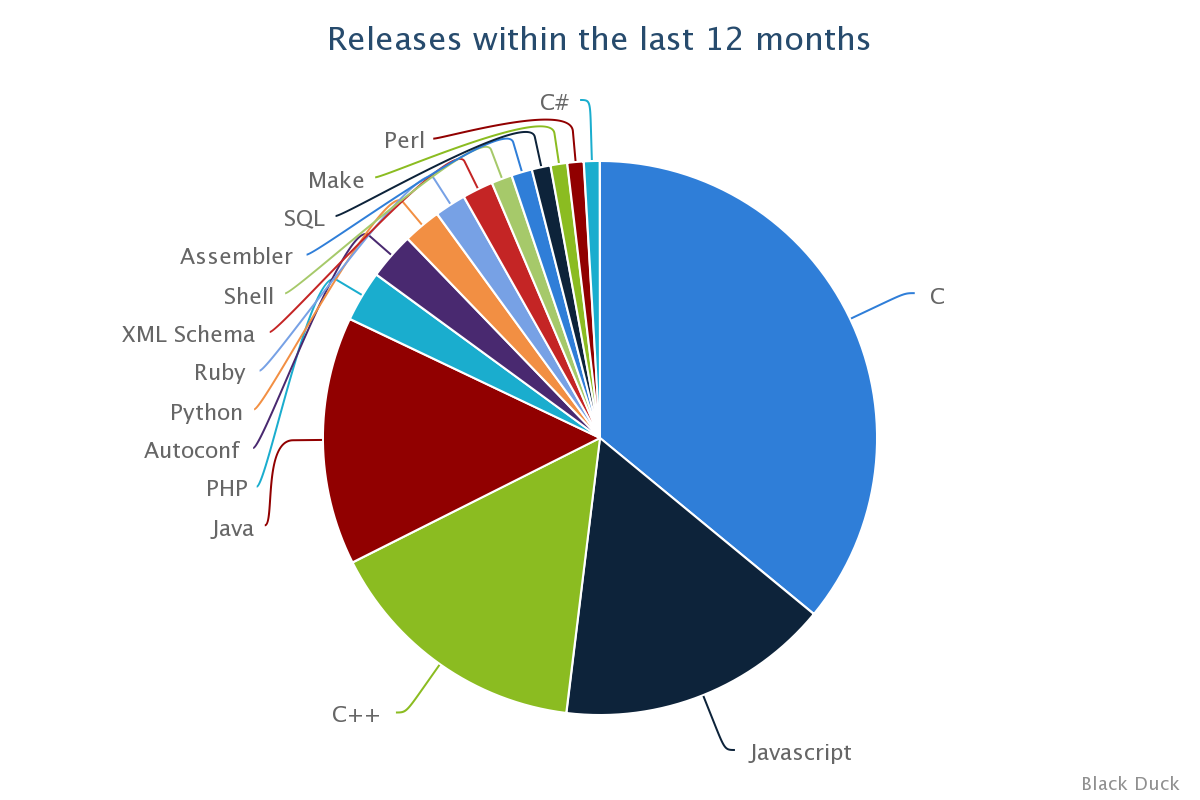
\includegraphics[width=0.9\linewidth]{../../data/js-trends/black-duck-15}

% \begin{figure}[h!]
% \begin{tikzpicture}
% [
%     pie chart,
%     slice type={c}{gray1},
%     slice type={js}{red},
%     slice type={cpp}{gray2},
%     slice type={java}{gray3},
%     slice type={php}{gray4},
%     slice type={autoconf}{gray5},
%     slice type={python}{gray6},
%     slice type={ruby}{gray1},
%     slice type={xml}{gray2},
%     slice type={sh}{gray3},
%     slice type={asm}{gray4},
%     slice type={sql}{gray5},
%     slice type={make}{gray6},
%     slice type={perl}{gray1},
%     slice type={csharp}{gray2},
%     pie values/.style={font={\small}},
%     scale=2
% ]

% \pie{}{%
%   34.80/c,%
%   15.45/js,%
%   15.13/cpp,%
%   14.02/java,%
%   2.87/php,%
%   2.65/autoconf,%
%   2.15/python,%
%   1.77/ruby,%
%   1.73/xml,%
%   1.18/sh,%
%   1.16/asm,%
%   1.07/sql,%
%   0.94/make,%
%   0.92/perl,%
%   0.90/csharp,%
% }

% \legend[shift={(1.3cm,0.9cm)}]{%
%   {C}/c,%
%   {Javascript}/js,%
%   {C++}/cpp,%
%   {Java}/java,%
%   {PHP}/php,%
%   {Autoconf}/autoconf,%
%   {Python}/python,%
%   {Ruby}/ruby,%
%   {XML Schema}/xml,%
%   {Shell}/sh,%
%   {Assembler}/asm,%
%   {SQL}/sql,%
%   {Make}/make,%
%   {Perl}/perl,%
%   {C\#}/csharp,%
% }
% \end{tikzpicture}
% \caption{Compilation results distribution}
% \end{figure}

\paragraph{Jobs}

The software industry is rather closed sourced, and its activity is rather opaque.
All these previous metrics are representing the visible activity about programming language, but are not representative of the software industry.
%To get a hint on the popularity of programming languages used in the software industry, the trends on job propositions are insightful.
The trends on job openings gives an hint of the direction the software industry is heading towards.
\textit{Indeed} provide some trends over its database of job propositions.
Javascript developers ranked at the third position, right after SQL and Java developers.
Then come C\# and C developers.
This position means that Javascript might finally be on the edge to become a major language in the software industry, and become as important as Java and C/C++.

\nt{TODO redo this graph, it is ugly.}
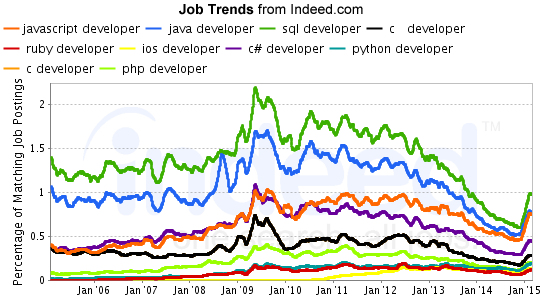
\includegraphics[width=0.9\linewidth]{../../data/js-trends/jobgraph}



All these metrics in this section represent different faces of the current situation of Javascript adoption.
With the rise of web applications, we can safely say that Javascript is one of most important language of this decade, alongside with Java and C/C++.
It is widely used in open source projects, and everywhere on the web, as well as in the software industry.

\section{Highly concurrent web servers}

\subsection{Concurrency}

\subsubsection{Scalability}

The internet allows interconnection at an unprecedented scale.
There is currently more than 16 billions devices connected to the internet, and it is growing exponentially\ftnt{http://blogs.cisco.com/news/cisco-connections-counter}.
This massively interconnected network gives the ability for a web applications to be reached at the largest scale.
A large web application like google search receive about 40 000 requests per seconds.
That is about 3.5 billions requests a day\ftnt{http://www.internetlivestats.com/google-search-statistics/}.
This traffic is huge, but it remains sensibly stable because the position of Google is assured.

% To handle such amount of traffic, Google deploys specific infrastructures, and software.

However, the traffic at the beginning of a web application is much more uncertain.
If the service propose a good service, it might become viral at some point because it is efficiently relayed in the media.
As a concrete example, when a web application appears in the evening news, it might expect a huge spike in traffic.
But most of the time, the spikes are unpredictable.

A young web application needs to follow the growth of its audience.
This growth might be steady enough to be planned, or it might be unexpected and challenging to meet.
Scalability is the ability for a web application to adapt its load to the demand in a reasonable time.

Scalability mainly holds on the ability of a web application to requests many concurrent requests.
For this thesis, I reduce scalability to concurrency.
A server is highly scalable if it is highly concurrent.
\comment{TODO better explanation of this simplification}
A highly concurrent server is able to manage a large number of simultaneous request.
It represent an uninterrupted flow of requests, with a growing throughput.
With the growing number of connected devices on the internet, concurrency is a very important property in the design of web servers.
As examples, around the year 2000, Dan Kegel wrote about the C10K\ftnt{http://www.kegel.com/c10k.html} problem.
How to handles 10K simultaneous connection on a web server.
More recently, in 2013, Robert Graham wrote about the C10M\ftnt{http://c10m.robertgraham.com/p/manifesto.html} problem.

\subsubsection{Tow faces of concurrency}

Concurrency is the ability for an application to make progress on several tasks at the same time.
It can be achieved either by parallelism, or by time-slicing concurrency.

The term Parallelism refers to techniques to make programs faster by performing several computations in parallel. This requires hardware with multiple processing units. Such hardware is nowadays omnipresent.
\ftnt{https://wiki.haskell.org/Parallelism_vs._Concurrency}

However, concurrency can be achieved on a single processing unit as well.
The executions of the different tasks are interleaved in time.
As an example, it is used to give multi-tasking ability to operating systems. 

Concurrency allows to stretch the computation on one, or many cores.
It enables scalability.
\comment{TODO review that}.

Parallelism improves performances for computation at a price.
It is necessary for the concurrent tasks to be independent.
Otherwise, two tasks could modify a shared state simultaneously resulting in a corrupted state.

In time-slicing concurrency, the concurrent tasks can more or less benefit of a shared state, depending on the scheduling strategy.
In this thesis I focus on the cooperative scheduling used in the event-loop.
It allows for a truly global memory and seems to be one of the easiest way for developers to write concurrent programs efficiently.
Indeed, I presented in the previous section the popularity of Javascript, which uses this scheduling strategy.

The other main scheduling strategy is preemptive scheduling.
It is used in most execution environment in conjunction with multi-threading.
However, it is known to be hard to manage, and should be avoided except when true concurrency is needed in concert with true shared state.
Shared state could probably always be emulated with isolated memory and message passing.

\subsection{Technological shift}

\subsubsection{Power wall}

Around 2004, the so-called Power Wall was reached.
The clock of CPU is stuck at 3GHz because of the inability to dissipate the heat generated for higher frequencies.
Additionally, the parallelism inside the stream of instructions is limited.
Because of these limitations, a processor is limited in the number of instruction per second it can execute.
Therefore, parallelism is the only option to achieve high concurrency.
And with parallelism, the isolation of the memory of each independent task.

\subsubsection{The case for global memory}

The best practice in software development advocates to design a software into isolated modules.
By following the best practice, the code base is split into modules.
Modularity allows to understand each module of the application by itself, without an understanding of the rest.
And to understand the application as the interconnections between modules.
The principles are encapsulation, a module contains the data, and the functions to manipulate this data ; separation of concerns, each module should have a clear scope of action, and it should not overlap with other scopes ; and loose coupling, each module should require no, or as little as possible knowledge about the definition of other modules.
The main goal followed by these principles, is to help the developer to develop and maintain a large code-base.

Modularity is intended to avoid a different problem than the isolation required by parallelism.
The former intends to avoid unintelligible spaghetti code.
While the latter avoids conflicting memory accesses resulting in corrupted state.
The two goals are overlapping in the design of the application.
Therefore, any language needs to provide a compromise between these two goals.

I argue that the more accessible, hence popular programming languages choose to provide modularity over isolation.
They provide a global memory at the sacrifice of the performance of provided by parallelism.
The more efficient languages sacrifice the readability and maintainability, to provide a model closer to parallelism, to allow better performances.
\comment{TODO here I use language in both cases, it would be better to use a more generic term to refer to language or infrastructure}

\subsubsection{Rupture}

Between the early development, and the mature development of a web application, its needs are radically different.
In its early development, a web application needs to quickly get feedback from its users.
The first reason of startup failures is the lack of market need\ftnt{https://www.cbinsights.com/blog/startup-failure-post-mortem/}.
The development speed is crucial.
Therefore, the development team opt for a popular, and accessible language.
The development team quickly releases a Minimum Viable Product as to get these feedbacks.
\textit{``Release early, release often''}, and \textit{``Fail fast''} are the punchlines of the web entrepreneurial community.

As the application matures and its audience grows, the focus shift from the development speed to the scalability of the application.
The ability of the application to handle a large amount of simultaneous request.
The development team then shift for a language providing parallelism.

From this shift derives two problems.
The first is that this shift is a risk for the future of the application.
It usually implies for the development team to rewrite the code base to adapt it to a completely different paradigm, with imposed interfaces.
It is hard for the development team to find the time, hence the money, or the competences to operate this shift.
Indeed, the number two and three reasons for startup failures are running out of cash, and missing the right competences.
The second problem is that after this shift, the development pace is different.
Parallel languages are incompatible with the commonly learned design principles.
The development team cannot react as quickly to user feedbacks as with the first paradigm.

% There is a performance problem with languages about concurrency.
% The used imperative programming languages are difficulty parallel.
% And the highly parallel programming languages are not largely used.

% There is a technological rupture between the two.

The technological rupture operated during the evolution of a web application is the demonstration that economically, there is a need for a language that exposes a more sustainable abstraction.
An abstraction that it is easy to develop with, like in the beginning of a web application development, and yet parallelizable, so as to be scalable when the application matures.

\subsection{A problem of memory}

The problem I focus on is the coordination of state between the concurrent execution in concurrent programming.
Precisely, I focus on a solution to leverage parallelism while keeping the global memory for developers.

I presented earlier the three main strategies to manage the memory in concurrent programming.
The main difference for the developer is how each model exposes the assurance of an invariance in the memory state.
I call invariance the assurance given to the developer that the global state of the application is not corrupted by the coordination between the concurrent executions.

In applications composed of multiple parallel processes, the memory of each processes is exclusive.
The developer is aware that only the process can modify its memory.
The processes propagate a modification to the state of the application by sending messages.
Each process treat these messages one after the other.
There is no risk of corrupted state by simultaneous, conflicting accesses.
The invariance is explicit because the memory is isolated inside each process.

In applications composed of multiple parallel threads, the memory is shared between all the threads.
The developer is aware that because of the preemptive scheduling strategy, the shared memory states of the application can be modified at any time by any thread.
To prevent conflicting accesses on the memory, the developer locks every shared memory state during a modification.
The developer assures itself the invariance of the memory.

In application using cooperative scheduling on an event-loop, like Javascript, the memory is global.
All the events are executed sequentially, so there is no possible simultaneous memory access.
The developer is aware of the points where the scheduler switches from one concurrent execution to the other, so it can manage its state in atomic modification.

The invariance exposed by the isolated processes and the event-loop are similar.
The developer defines sequence of instructions with atomic access to the memory.
And in both paradigms, these sequences communicate by sending messages to each other.
The difference lies in the isolation of this memory.
\comment{TODO this paragraph needs review}

I argue that the language should adapt to the developer and expose a concurrent paradigm with a global memory.
Then a compiler, or the execution engine, can isolate the memory so as to parallelize the concurrent executions.
So as to provide to the developer a usable, yet efficient compromise.

\section{Compilation}

We propose to find an equivalence between an event loop and a network of isolated processes.
This equivalence should allow a compiler to transform an event loop into several parallel processes communicating by messages.

With this compiler, it would be possible to express an application with a global, so as to follow the design principles of software development.
And yet, the execution engine could adapt itself to any parallelism of the computing machine, from a single core, to a distributed cluster.

This equivalence intend not to be universal.
It focuses on a precise class of applications : real-time Web applications processing stream of requests from users.

\subsection{Real-time web services}

Web applications are now written in a stream fashion.
Indeed, as I showed previously, the event loop is executed like a pipeline.
Web services can be seen as pipelines processing streams of requests.

In a stream processing application, there is roughly two kinds of usage of the global memory : data and state.
Naively, the data represent a communication channel between different point in the application space, and the state represents a communication channel between different instant in time.
The data flow from stage to stage through the pipeline, and are never stored on any fluxion.
The state, on the other hand, remains in the memory to impact the future behaviors of the application.
State might be shared by several parts of the application.

There are different kinds of state dependencies in applications components leading to different kinds of parallelism.
In this thesis I argue that it is possible to parallelize a real-time web applications written on an event-loop because the strong dependencies mainly remains within a closed number of concurrent executions.

\endinput



\subsubsection{Learning curve}

Because the compiler intend to warn the developer about shared states, it would be a great tool for beginner to progressively adapt to the flow programming model and best practices.


\subsubsection{Granularity of abstraction}

Finally, the difference of memory isolation is the result of two different granularity of abstraction.

The granularity of the machine is not the same as the granularity of the program.
You hardly have the same number of request as the number of processors.
The developer wants to be presented with an abstract machine.

We argue that, provided the compiler to split the memory, an event-loop is a good fit for this abstract machine.
This abstract machine being the `good` representation for the developer of the underlying machine.




\subsubsection{Performance reason}
Global memory increase performances when there is single threads.
Functional languages with immutability exists since a long time.
It allows a good memory isolation, and thus, parallelism.
But, if it is conceptually elegant \comment{please argument here}, it needs deep copies which is bad for performances.
The argument here is that when there is no parallelism, a global memory is better.
So the isolation of the memory should be driven by the need for actual parallelism, not potential parallelism.
So, the loss of performance due to copying, or wire transfer, is compensated by the parallelism.





This scale translates into many different design implementation.
We present here three representative alternatives.

\paragraph{Multi-thread} %  // Data parallelism

In the multi-thread paradigm, each request is mapped onto a thread to be executed independently.
On a multi-core architecture, multiple thread can progress at the same time.
However, if they need the same resources, they need to share them.
To assure there is no concurrent access on these resources, they lock the resources while they use them to disallow other threads to modify them.
However, when there is a large amount of requests, this locking strategy is counterproductive.

\paragraph{Pipeline} %  // Task parallelism

The pipeline paradigm split the processing of a request into many stages.
These stages are independent, they don't share anything, so they can be executed in parallel without lock.
However, it imposes the developer to write its application as a sequence of isolated stages.

\paragraph{Event-loop}

An event-loop process requests sequentially.
% which allows to keep a global memory.
As only one request is executed at once, it has exclusive access to the memory.
Therefore, it allows to share state across the application without lock mechanism.


The first two leverage parallelism.
They can stretch the execution on multiple cores.
The last one is sequential, and is restrained on one core.
Yet, we show that this last model is easier to develop because of this global memory.






\subsection{Liquid IT}

The goal of Liquid IT is to hide the technical complexity of scalability to the developer, so he can focus solely on business logic.




TODO Talk about the annotations used by many parallel languages.





-------
They require only a few machines.
As a comparison, a smartphone, or a laptop could suffice.
The technologies to start developing an application are available to anyone, and require reasonable knowledge.
There is numerous resourceson the internet to learn the languages detailed in the previous section, and start releasing a web application.

Between the infrastructure needed, and the technologies to grasp, there is a huge technological contrast between the beginning of a web application, and its massive success.

With virtualization of servers it is possible to ...
--------




% But many large company replaced the initial languages of the web with scalable solutions.
% Twitter : Ruby -> Storm
% Facebook : PHP -> HHVM / Flux ...
% Google : MapReduce, Kubernetes, Borg ...






I think, there is not a decisive difference between the infrastructure and the language, Node.js, or the DOM are what placed Javascript where it is now.
And Erlang is a language, not an infrastructure, and yet, it suffers from the same problems than most infrastructures.
These corner cases make me believe the difference is not between language and infrastructure, but holds in two characteristics at the core of the interfaces proposed by languages or infrastructures.

The first characteristic is how the machine is represented by the language.
This characteristic, is indeed really close to the difference language infrastructure, as language tends to abstract the machine, while infrastructure tends to provide direct accesses for the developer.
Does the developer manipulate concrete representation of the underlying machine, like execution containers process, thread, actors, and so on ...
Or does it manipulate abstract representation, like a global key values store,memory, references, functions and so on ...

Are these representations continuous, or discrete ?

\paragraph{The representation of the execution}
A pool of thread is discrete, there is a finite number of thread.
While in a functional language, the number of function is more continuous.
Specifically, the number of functions / modules, depends only on the structure of the program and the needs of the developer.
A program can contains as many functions / modules as it needs, it doesn't impact the performance.
While the developer is more limited in the number of threads, because it directly impact the performances, or has incentives to deal with threads to augment the performance.

Concurrency is an abstract representation, it doesn't imply specifically that there are parallel executions, or time-sliced executions.
It simply express the dependencies between different steps in the execution.
Parallelism on the other hand tends to be a more concrete representation as it is intended to be executed simultaneously.

\paragraph{The representation of the memory}







Performances comes from one factor : parallelism.
The only factor that comes in play, is how a language / infrastructure present this parallelism to the developer.
Most choose to give direct access to the developer : actors, threads, process ... mostly infrastructures and erlang.
Other choose to give no access, at the cost of completely loosing parallelism : imperative languages without the infrastructure.

This parallelism needs to exploit tow aspects.
- execution representation : unique, multiple.
How the dependencies are expressed between operations.
- memory representation : global, isolated.
How the executions depends on the memory.

Unique execution, global memory : imperative

Multiple execution, global memory : threads

Unique execution, isolated memory : OOP ?

Multiple execution, isolated memory : Actors / process ...


We see that multiple executions are mostly a fail.
So the developer needs to have an abstract representation of an unique  execution, that will be split at compilation or execution.
See about the continuity (scalability) of the execution model.

To allow the split of execution, we needs hints about the dependencies between operations, both in term of causality, and in term of memory share.

Cooperative scheduling successfully allow to represent the dependencies between operations.

However, as soon as the developer is not aware anymore of the invariance, it fails, because it needs explicit synchronization (locks), which are a pain to manage.

Instead, I think the sweet spot is in letting the developer provide the invariance via cooperative scheduling.

"                               IMPORTANT                                     "
Multiple execution are difficult to manage, only because it implies to manage the coordination of state.
Either via isolation and messages, or sharing and locking.
"                                                                             "

\paragraph{The invariance}

The invariance, is how the language let the developer know the integrity of the memory, while still letting her choose points of rupture to allow parallelism.

There is a scale between explicit synchronization of variables (locks) and implicit atomicity of execution on the global memory (cooperative scheduling).
The granularity is not the same, in terms of execution and memory :

          execution                      memory
        ---------------------------------------------------------------
lock :    small granularity (region)     small granularity (variable)
coop :    large granularity (event)      large granularity (global memory)

what about the two other kind

          small granularity              large granularity     ->    ?
          large granularity (actor)      small granularity     ->  actors




Threads are pre-emptive.
Fibers, green threads and so on are pre-emptive. (they are cooperatively scheduled, but they don't let the developer know when they are cooperatively scheduled)
The event-loop is not.

Global memory :

The fundamental difference is in the control they allow to the developer.
The event-loop abstract some stuffs (to define, but basically the threads, or the scheduling), and gives access to other stuffs : the pre-emption.
The threads, green threads and so on abstract the pre-emption, while they give access to the granularity of parallel executions.

Because of this pre-emption, to assure the invariance, threads provided the solution of locks.
But it is difficult to manage and leads to deadlock.
It is a degenerated version of the solution of atomic execution provided by the event-loop : you have complete access on the memory, and you won't be pre-empted.

Isolated memory :

Actors and processes, like the threads, allow you to split the execution 

 gives you another kind of control on the memory






How the developer needs to protect the memory invariant from pre-emption in different concurrency models ?
  event-loop  |  thread  |   process
     none     |  locks   |  isolation

-> So when developers are in control of the pre-emption, they manage it safely.
(compared to when they have to assure locks, or isolation)


How parallelizable is the model ? So how scalable is it ?
  event-loop  |  thread  |   process
       0      |     +    |     +++

-> So isolated process are the way to go for parallelism.
(It is the only true parallelism indeed)

So the sweet spot is a compiler from event-loop to process.


Event-loop is perfect for real-time web application.
Application processing stream of data.
So it is possible to compile real time web application using-event loops into chain of processes.



Explosion of Javascript popularity

Turn-based programming
  -> Javascript is turn based, it is a better solution than threads, and process for concurrency.






\begin{center}
\rule{4cm}{0.4pt}\\
old stuffs\\
\rule{4cm}{0.4pt}
\end{center}



\subsection{Separation of concerns}


% I see a trend here.
% http://pchiusano.blogspot.fr/2010/01/actors-are-not-good-concurrency-model.html

The languages presented in the last section all have large developing community. Some are functional, others are object-oriented.

To answer the first question.
If a module is limited inside an actor, then the reusability of the module is te be questioned.
It loses its point as a generic component, reusable through the codebase.
Or it is stateless.
Or its state is boundable by the actor.

To answer the second question.
For a module to be composed of actors, means that the messages the actors receive contains somehow information about the context they are executed.
That is, at least, the actors to get the result back.

So, in some extents, it is possible to establish an equivalence between modules and actors. However, the transition is too tedious to be done manually.
That is why most web applications neglect the module approach to adopt the actor approach, when true scalability is needed.
At the lost of the development ease.


% Functional programming isolates the scope of effects for the program to be 
But they all provide some ways to apply the separation of concerns principle : modules.
Think of a module as an object in OOP, or a monad(?) in FP.

It assure that the behavior of a module is completly contained in this module, and does not depends on external parts.
Splitting a large program into many modules allow developers to safely modify a module only by understanding itself, and its interface.
It is the divide and conquer strategy, applied to computer science.
% Separation of concerns. TODO read these :
% - http://en.wikipedia.org/wiki/Separation_of_concerns
% - http://deviq.com/separation-of-concerns/
% - http://stackoverflow.com/questions/98734/what-is-separation-of-concerns
% - http://c2.com/cgi/wiki?SeparationOfConcerns

The separation of concerns principle incites to design simple, generic, reusable modules. 
Some modules can provide more complex behavior, by relying on, and composing with other modules.
The separation of concern incite to develop modules to be generic.
It must be independent from where, and how it is used, to be able to be reused.
De facto, a module is meant to be disseminated through the code base of the program.
Implying that if the module rely on some state, this state must be available in a global memory, and that there is no concurrent access.

This principle allows to quickly develop, and maintain an application.
For a new web application to meet the requirements of its user community, it is crucial to be able to quickly modify its codebase.
\comment{I usually starts from this argument. But here I barely use it. TOOD integrate better this argument.}
% Moreover, it is possible to increase the development team, as the code base is divided into independant parts communicating via well-defined interfaces,
And that is why the development of most, if not all, web applications starts using language allowing with modularity.


\subsection{Performance Scalability}

% \comment{TODO I explain exactly what I mean by Development scalability (I should change the term, it is misleading and not explicit enough), and Performance scalability.}

% How to measure refactoring ease ?

Yet, because of the global memory used to centralize module state, while disseminating the module methods, it is difficult for this first approach to scale.
Indeed, scalability is known to come from parallelism, which is incompatible with a global, shared memory space.
\comment{TODO explain these shortcuts}
\comment{TODO explain the invariance and parallelism. The developer provides insight about parallelization by manipulating the points where invariance of the state is assured. Isolation, locks, or yields}.

At some point, the development team discard this first approach, for a distributed execution model.
Such model distribute the execution onto different computers communicating by messages.
\comment{To simplify the argument, I called these isolated computers, actors. TODO change that name.}
% To maximize the organization possibilities network of actors, it is important that an actor can send a message to any other actor.
The essence of an actor is to have only one execution thread, so as to isolate its state, and have exclusive access on it.
This exclusivity assure the invariance, without relying on synchronization mechanisms.
And if its state is isolated, there is no need to reduce the scope of this actor to reach other actors.
\comment{TODO this argument is not strong enough}

Actors are not composable the way modules are.
The different functions of a module are used in the call / return fashion while actors are used in the fire-and-forget fashion.
An actor sends its result to another actor, than the one which sent the initial message.
It is not possible to compose an actor, like it is possible for a module.
That is, it is not possible to use an actor in different contexts.


The best way to assure parallelism is through isolation.
Yet, the way that developers seems to find most appealing to assure concurrency is through cooperative scheduling aka event-loops.
We observe that there is no large community around languages/frameworks providing isolation.
But there is large communities around languages/frameworks with event-loops.

\subsection{A universal language : the holy Graal}

% \comment{TODO assure transition, explain more about this argument}
% Therefore, it is important to decouple the physical resources used during the execution, and the modularity used to develop the application.

Is it still possible to combine the advantages of modules, with the advantages of actors ?
Is it possible for modules to extend beyond the boundaries of actors, using message-passing, instead of global memory for coordination ?
And is it possible for a module to be composed of actors ?

To answer the first question.
If a module is limited inside an actor, then the reusability of the module is te be questioned.
It loses its point as a generic component, reusable through the codebase.
Or it is stateless.
Or its state is boundable by the actor.

To answer the second question.
For a module to be composed of actors, means that the messages the actors receive contains somehow information about the context they are executed.
That is, at least, the actors to get the result back.

So, in some extents, it is possible to establish an equivalence between modules and actors. However, the transition is too tedious to be done manually.
That is why most web applications neglect the module approach to adopt the actor approach, when true scalability is needed.
At the lost of the development ease.


% Functional programming isolates the scope of effects for the program to be more readable -> it is roughly separation of concern.
% Parallelism needs isolation to avoid race conditions and state corruption.

% You want to isolate a module to be able to understand it, only by looking at its code, and not the whole codebase. But you want it to be reused in many places in the code.

% You want to isolate an actor so that it can have exclusive access to its state.
% But you want it to be able to reach any other actor.





\comment{TODO why ?}


The transposition from the module organization, to the actor organization is a tedious process, and should be handled by a compiler.
Therefore, to have both performance through parallelism and still attract a large developer community, we need to find an equivalence between the module organization, and the performance point of view on parallelism.

\comment{TODO now talk about the limitations of this transition. you mention earlier that actors need to receive information about their context, and that modules needs to be stateless, or that their states needs to be bounded by the actor.}

So the hypothesis is : by providing a tool to transform the invariance of cooperative scheduling into isolation and message-passing, it should be possible to provide a developer-friendly scalable paradigm.
\comment{I don't know if hypothesis is the right term for this assumption}

This transformation is done by isolating the memory use by each atomic execution of the event-loop (the callbacks).
But this isolation is not possible for every kind of application.
Applications could be classified in the level of coordination necessary in their design. (See below for a classification from Gunther's Universal Scalability Law)
At a very end of the spectrum, there is static content servers, where there is no coordination, everything is parallel.
At the very other end of this spectrum, there are consistent databases, where the coordination require the application to be highly sequential.

Web applications that are designed in a certain way (flow-based web applications -> no retropropagation) are in the middle of this spectrum.
We advance as the thesis that it is possible for these types of web applications to isolate the memory for each atomic execution of the event-loop (the callbacks).



The different kind of applications, from Gunther's Universal Scalability Law (USL) :
Application classes for the USL model.

\begin{tabular}{c|l} \hline

\multirow{4}{*}{A} & \textbf{Ideal concurrency} ($\alpha, \beta = 0$)      \\
                   & Single-threaded tasks                                 \\
                   & Parallel text search                                  \\
                   & Read-only queries                                     \\ \hline
\multirow{4}{*}{B} & \textbf{Contention-limited} ($\alpha > 0, \beta = 0$) \\
                   & Tasks requiring locking or sequencing                 \\
                   & Message-passing protocols                             \\
                   & Polling protocols (e.g., hypervisors)                 \\ \hline
\multirow{3}{*}{C} & \textbf{Coherency-limited} ($\alpha = 0, \beta > 0$)  \\
                   & SMP cache pinging                                     \\
                   & Incoherent application state between cluster nodes    \\ \hline
\multirow{4}{*}{D} & \textbf{Worst case} ($\alpha, \beta > 0$)             \\
                   & Tasks acting on shared-writable data                  \\
                   & Online reservation systems                            \\
                   & Updating database records                             \\ \hline
\end{tabular}
\\~\\












\section{Proposal and Hypothesis}

\subsection{LiquidIT}

A general definition of Liquid IT.
And more specifically the focus on dev and perf scalability.
Liquid IT should try to bring a solution to this compromise leveraging the particular position of Javascript and its event-loop.


\subsection{Parallelization and distribution of web applications}
% \subsection{Pipeline parallelism for event-loop}


\subsection{\comment{Hypothesis and Thesis}}




%-----------------------------------------------------------------------------%
                                    \endinput
%-----------------------------------------------------------------------------%


Some links I NEED to put :
--------------------------

https://glyph.twistedmatrix.com/2014/02/unyielding.html
http://calculist.org/blog/2011/12/14/why-coroutines-wont-work-on-the-web/


Some chunks I might find useful later :
---------------------------------------

\cit{No matter how great the talent or efforts, some things just take time. You can't produce a baby in one month by getting nine women pregnant.}
{Warren Buffett}

A good example of declarative sentence in everyday world : in case of fire, 
the elevators don't work -> you understand that you need to take the stairs.

The purpose of explicit synchronization is to manage the timing of side-effects in the presence of parallelism. 

A function is side-effect free if it is referentially transparent.




Why is that cooking recipe are inehrently and easily parallel, while it is a lot more difficult to write parallel programs ?

The intuitive understandings of the scope of side-effects.
In a recipe, it is easy to understand what each steps do, and how it might interfere with others, or which are required by others.
With the naivete of computers, every interaction needs to be explicitely defined to avoid conflict.
And with the size of programs, it is important to keep these interactions to a minimum.

While in a computer program, it is a lot more difficult.
It boils down to have boundaries in your system, and coordination to articulate the parts.

The two extremes are functional programming, message passing, actor model, multi-process, with statelessness, side-effects free, referential transparency ...
\comment{TODO there is HUGE differences between all these concepts. The common point is isolation of memory in space (rather than time with the following solution), but in terms of composition, functional programming and every other, are completly different. FP allows composition (the same point handle call and returns, a single point of connection), which is not true to message passing and so on ...}
And Shared memory multi-threading, with locks, transaction memory ...
Which basically isolate memory in time.





The original explanation :
--------------------------

Languages with parallel execution features are not mainstream, because it is difficult to provide a good way for the developer to coordinate between the different parallel executions.
The two main current designs for this coordination are synchronization mechanims for threads, or isolation for processes.
Both are pretty difficult to manage.
It is known that synchronization is difficult. \comment{TODO Develop this further, with arguments}
And as we see from many parallel languages or frameworks, isolation-based coordination never really took off. Probably because it is too difficult for most programmers to efficiently manage both the isolation, and the features organization.
\comment{TODO a better explanation is needed here (inspiration from the abstract), and some solid arguments}

These two methods assure to the developer the invariance in the memory.
If we step back from parallelism, into all concurrency, we have three methods to assure this invariance :
\begin{itemize}
\item Synchronization mechanisms are used by threads to assure that no other threads is using a common memory region : it assure the invariance of this memory region during the execution. But it is known to be difficult to develop scalable applications with such mechanisms.
\comment{TODO develop this with arguments, maybe merge with above}
\item Isolation is another way to assure the invariance : each process is sure to have exclusive access to its memory, and therefore, it assure the invariance.
It is used by parallel frameworks, but it require the developer to think both at feature modularization and isolation.
We suppose that the two are not easily conciliable, and that is why we observe that isolation-based languages and frameworks never really took off.
\comment{TODO arguments}
\item Exclusive atomic execution is a third way to assure invariance. It is used by the Javascript event-loop. It assure that a) each execution is atomic until it yield b) the developer is aware of this yielding, and acknowledge the invariance between the yields.
But as the execution is localized to keep a global memory, it is not parallel and therefore, not scalable.
\end{itemize}

There is two different levels here.
The developer point of view seems inconsiliable with the performance point of view.

From the developer end, the best way for developer to easily acknowledge this invariance in a concurrent execution seems to be through sequential atomic and exclusive executions : Cooperative scheduling, like used by the event loop.
But this cooperative scheduling must remain managed by the developer (at least for the moment), therefore, it is important to keep keyword like yield, and so, and not rush into the green thread paradigm \comment{see the article unyielding on deciphering glyph's blog}.
The memory is global (to assure coordination), but accessed in turns.

From the performance end, the best way to assure scalability is through a parallelism based on isolation, and message-passing.
The memory is splitted in isolated and exclusive portions, with messages to assure the coordination.
\comment{TODO argue why it is the best way}

Therefore, to have both performance through parallelism and still attract a large developer community, we need to find an equivalence between the developer point of view on the invariance, and the performance point of view on parallelism.

So the hypothesis is : by providing a tool to transform the invariance of cooperative scheduling into isolation and message-passing, it should be possible to provide a developer-friendly scalable paradigm.
\comment{I don't know if hypothesis is the right term for this assumption}

This transformation is done by isolating the memory use by each atomic execution of the event-loop (the callbacks).
But this isolation is not possible for every kind of application.
Applications could be classified in the level of coordination necessary in their design. (See below for a classification from Gunther's Universal Scalability Law)
At a very end of the spectrum, there is static content servers, where there is no coordination, everything is parallel.
At the very other end of this spectrum, there are consistent databases, where the coordination require the application to be highly sequential.

Web applications that are designed in a certain way (flow-based web applications -> no retropropagation) are in the middle of this spectrum.
We advance as the thesis that it is possible for these types of web applications to isolate the memory for each atomic execution of the event-loop (the callbacks).



The different kind of applciations, from Gunther's Universal Scalability Law (USL) :
Application classes for the USL model.

\begin{tabular}{c|l} \hline

\multirow{4}{*}{A} & \textbf{Ideal concurrency} ($\alpha, \beta = 0$)      \\
                   & Single-threaded tasks                                 \\
                   & Parallel text search                                  \\
                   & Read-only queries                                     \\ \hline
\multirow{4}{*}{B} & \textbf{Contention-limited} ($\alpha > 0, \beta = 0$) \\
                   & Tasks requiring locking or sequencing                 \\
                   & Message-passing protocols                             \\
                   & Polling protocols (e.g., hypervisors)                 \\ \hline
\multirow{3}{*}{C} & \textbf{Coherency-limited} ($\alpha = 0, \beta > 0$)  \\
                   & SMP cache pinging                                     \\
                   & Incoherent application state between cluster nodes    \\ \hline
\multirow{4}{*}{D} & \textbf{Worst case} ($\alpha, \beta > 0$)             \\
                   & Tasks acting on shared-writable data                  \\
                   & Online reservation systems                            \\
                   & Updating database records                             \\ \hline
\end{tabular}
\\~\\
